% Syslab Research Journal Template
% By Patrick White
% September 2019
% version 1.1 - 9/5/2019

% INSTRUCTIONS: Edit the file as appropriate and replace with your journal text. Do NOT edit
%							any section headers or titles, tabling commands, fonts, spacing, sizes, etc.

% -------  Do NOT edit this header
\documentclass[letterpaper,11pt]{article}
\usepackage[paperwidth=8.5in,left=1.0in,right=1.0in,top=1.0in,bottom=1.0in,paperheight=11.0in]{geometry}
\usepackage{palatino}
\usepackage{graphicx}
\graphicspath{ {./} }
\def\hrulefill{\leavevmode\leaders\hrule height 20pt\hfill\kern\z@}

% ------------- DO Edit these definitions ---------------------
\def\name{Mikail Khan}
\def\period{5}
\def\journalnum{6}
\def\daterange{9/2/19-9/6/19}
% ------------------ END ---------------------------------

% Do NOT edit this
\begin{document}
	\thispagestyle{empty}
	\begin{flushright}
		{\Large Journal Report \journalnum} \\
		\daterange\\
		\name \\
		Computer Systems Research Lab \\
		Period \period, White
		\end{flushright}
	\hrule height 1pt
% ------------------ END ---------------------------------%	
	
% ------------------- Begin Journal reporting HERE ---------------

% ------ SECTION DAILY LOG -------------------------------------
	\section*{Daily Log}

	\vspace{-0.5em}
		\subsection*{Monday October 7}

                I made the datastructures for storing graph data and got a graph of speed to appear when you right click a shape.
		
		\subsection*{Wednesday October 9}

                I set up a super basic GUI using a library and made a right click menu on clicking a shape that doesn't do anything. I also made screen sizing work a lot better. 

		\subsection*{Friday October 11}

                I redid how graphs work a bit and made them selectable from the right click menu. Right now you can graph speed, x velocity, y velocity, and rotational velocity. There are four colors but there's no legend or scale yet. I did the graphs through the game engine but it probably wouldn't be hard to switch to doing it through the gui library.
                \\[0.5cm]
                Screenshot included here to save space. I adjusted the colors to save ink. Red is the speed of the circle and green is its y-velocity. I had dropped it and let it bounce.\\
               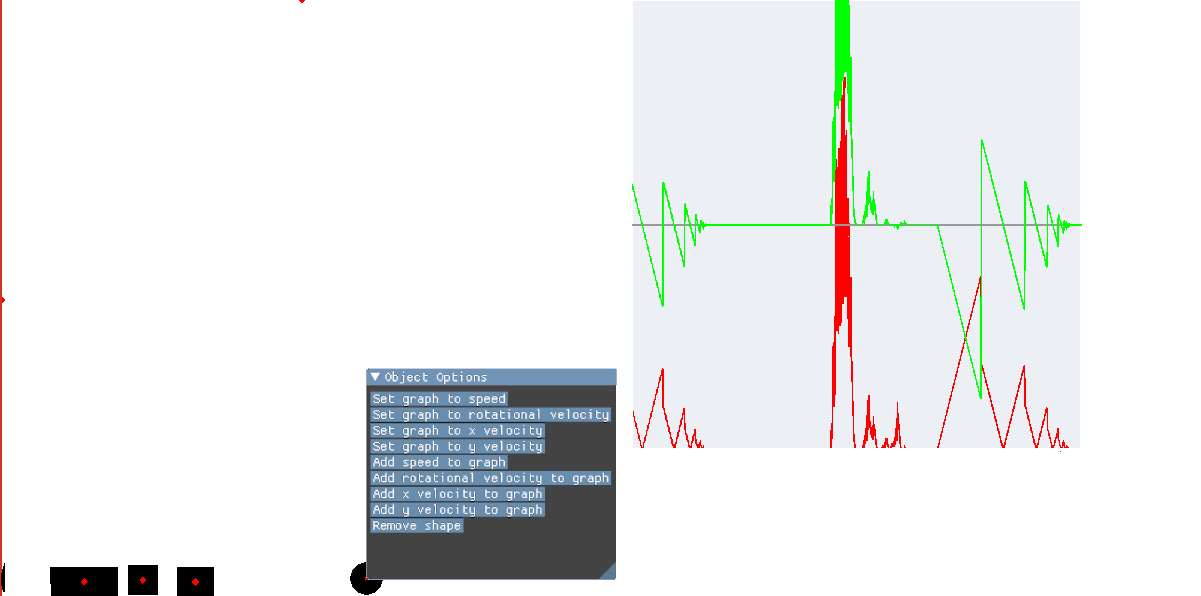
\includegraphics[scale=0.5]{screenshot}
	
% ------ SECTION TIMELINE -------------------------------------
	\newpage
	\section*{Timeline}
	\begin{tabular}{|p{1in}|p{2.5in}|p{2.5in}|}
		\hline 
	\textbf{Date} & \textbf{Goal} & \textbf{Met}\\ \hline
		\hline
		Today minus 2 weeks & CCD & Refactoring for CCD done\\
		\hline
		Today minus 1 weeks & CCD & CCD is done, but it doesn't solve the jittering/tunneling problem like I'd thought it would.\\
		\hline
		Today  & Graphs and improved UI & Yes, graphs work pretty well and I set up the GUI library in a way that should be pretty expandable\\
		\hline
                Today plus 1 week & Better simultaneous collision resolution & This might take a while and honestly I could spend the whole year on it. However, because circles work perfectly and they can probably illustrate everything needed to teach basic mechanics perfectly fine, I'll put this aside and only work on it in my free time if I can't get it working in two weeks. \\
		\hline
                Today plus 2 weeks & Complete UI and record graph data & A main UI including a help menu, object addition menu, export graph data, etc. Should be pretty much the end of this simulator, next was supposed to be electrodynamics and magnetism but I think I'll do either wave labs or universal gravitation first.\\
		\hline
	\end{tabular}


% ------ SECTION REFLECTION  -------------------------------------
	\section*{Reflection}
			In narrative style, talk about your work this week. Successes, failures, changes to timeline, goals. This should also
			include concrete data, e.g. snippets of code, screenshots, output, analysis, graphs, etc.

                        This week was pretty successful. Graphing was expectedly easy to implement and adding the GUI library was surprisingly easy. The GUI I have now isn't perfect but it definitely gets the job done. The graphs generated are also pretty informative; I can confirm that circles are perfect and e.g graphs of a thrown object's speed are a parabola. I might swith to using the GUI library for graphing so that the graphs are more easily resizeable and moveable but because I want to add things like graphs of vectors and FBDs drawing directly with the game engine gives me more control. I'll probably add a gui to create circles and rectangles this week but like always it will be a lot harder for custom convex polygons.

\end{document}
